%!TEX root = ../thesis.tex
%*******************************************************************************
%****************************** Third Chapter **********************************
%*******************************************************************************
\chapter{Manufacturing Technology of Power MEMS Devices}
\label{ch:Manufacturing Technology of Power MEMS Devices}

% **************************** Define Graphics Path **************************
\ifpdf
    \graphicspath{{Chapter6/Figs/Raster/}{Chapter6/Figs/PDF/}{Chapter6/Figs/}}
\else
    \graphicspath{{Chapter6/Figs/Vector/}{Chapter6/Figs/}}
\fi

In the Part II, I would systematically study the manufacture of GaN power MEMS devices from epitaxial growth \index{Epitaxial!growth} wafers \index{Wafer} to well-functional devices. Benefiting from the rapid development of III-V compound semiconductor fabrication and characterization equipment, various complex microstructures including GaN microcantilever \index{Cantilever} structures can now be easily realized by equipment devices with different functions. This chapter will introduce the main nanofabrication and characterization equipment, including epitaxial growth, dry \index{Etching!dry etching} etching, photolithography, thin \index{Photolithography} film \index{Thin film} deposition, plasma \index{Cleaning!plasma cleaning} cleaning, Raman \index{Raman!spectroscopy} spectroscopy, scanning electron \index{Scanning electron microscopy (SEM)} microscopy, transmission \index{Transmission electron microscopy (TEM)} electron microscopy, etc. I would briefly introduce their important role in GaN power MEMS \index{MEMS} research, as well as the corresponding process \index{Fabrication process} design and key parameters. The equipment mentioned in this chapter and later all belong to the micro-nano processing platform of the Chinese Academy of Sciences. The pictures of some of the equipment are from the official website of the equipment manufacturer, and all the models shown here are in one-to-one correspondence with the real objects.

\section{Fabrication techniques}

\subsection{GaN-on-Si wafer epitaxial growth}

\begin{figure}[H] 
\centering    
\includegraphics[width=0.8\textwidth]{MOCVD}
\caption[Aixtron CCS 3×2 MOCVD]{Aixtron CCS 3×2 MOCVD}
\label{fig:MOCVD}
\end{figure}

The GaN wafers \index{Wafer} are typically obtained by epitaxial growth \index{Epitaxial!growth} on Si substrates \index{Substrate} due to the less \index{Lattice!mismatch} lattice mismatch. Metal \index{MOCVD} Organic Compound Chemical Vapor Deposition (MOCVD), also known as Metal Organic Vapor Phase Epitaxy (MOVFE) is an important method for preparing nitride \index{Nitride} semiconductor materials, and it is also the most widely used method in the industry. MOCVD uses organic compounds of group III and group II elements and hydrides of group V and group VI elements as crystal \index{Crystal} growth source materials, and conducts vapor phase epitaxy on the Si substrate by thermal decomposition reaction to grow various III-V group, II-VI group compound semiconductors and their multicomponent solid solutions.

The growth of nitride crystals \index{Crystal} is usually carried out in cold-wall or hot-wall reaction chambers under normal or low pressure (\num{1e1} $\sim$ \num{1e5} \unit{\Pa}). In the \index{Epitaxial!growth} growth of GaN materials, trimethylgallium (\ce{TMG}) and ammonia gas (\ce{NH3}) carried by \ce{H2} are usually injected into the reaction chamber at the same time, and the reaction gases are transported to the surface of the high-temperature substrate \index{Substrate} and mixed above. The chemical reaction occurs as follows:
\begin{equation}
\mathrm{Ga}\left(\mathrm{CH}_{3}\right)_{3} \text { (gas) }+\mathrm{NH}_{3} \text { (gas) } \rightarrow \mathrm{GaN} \text { (solid) }+3 \mathrm{CH}_{4} \text { (gas) }
\end{equation}
the resulting GaN molecules are deposited on the surface of the Si substrate to form an epitaxial film \cite{hao2016nitride}.

\begin{figure}[H] 
\centering    
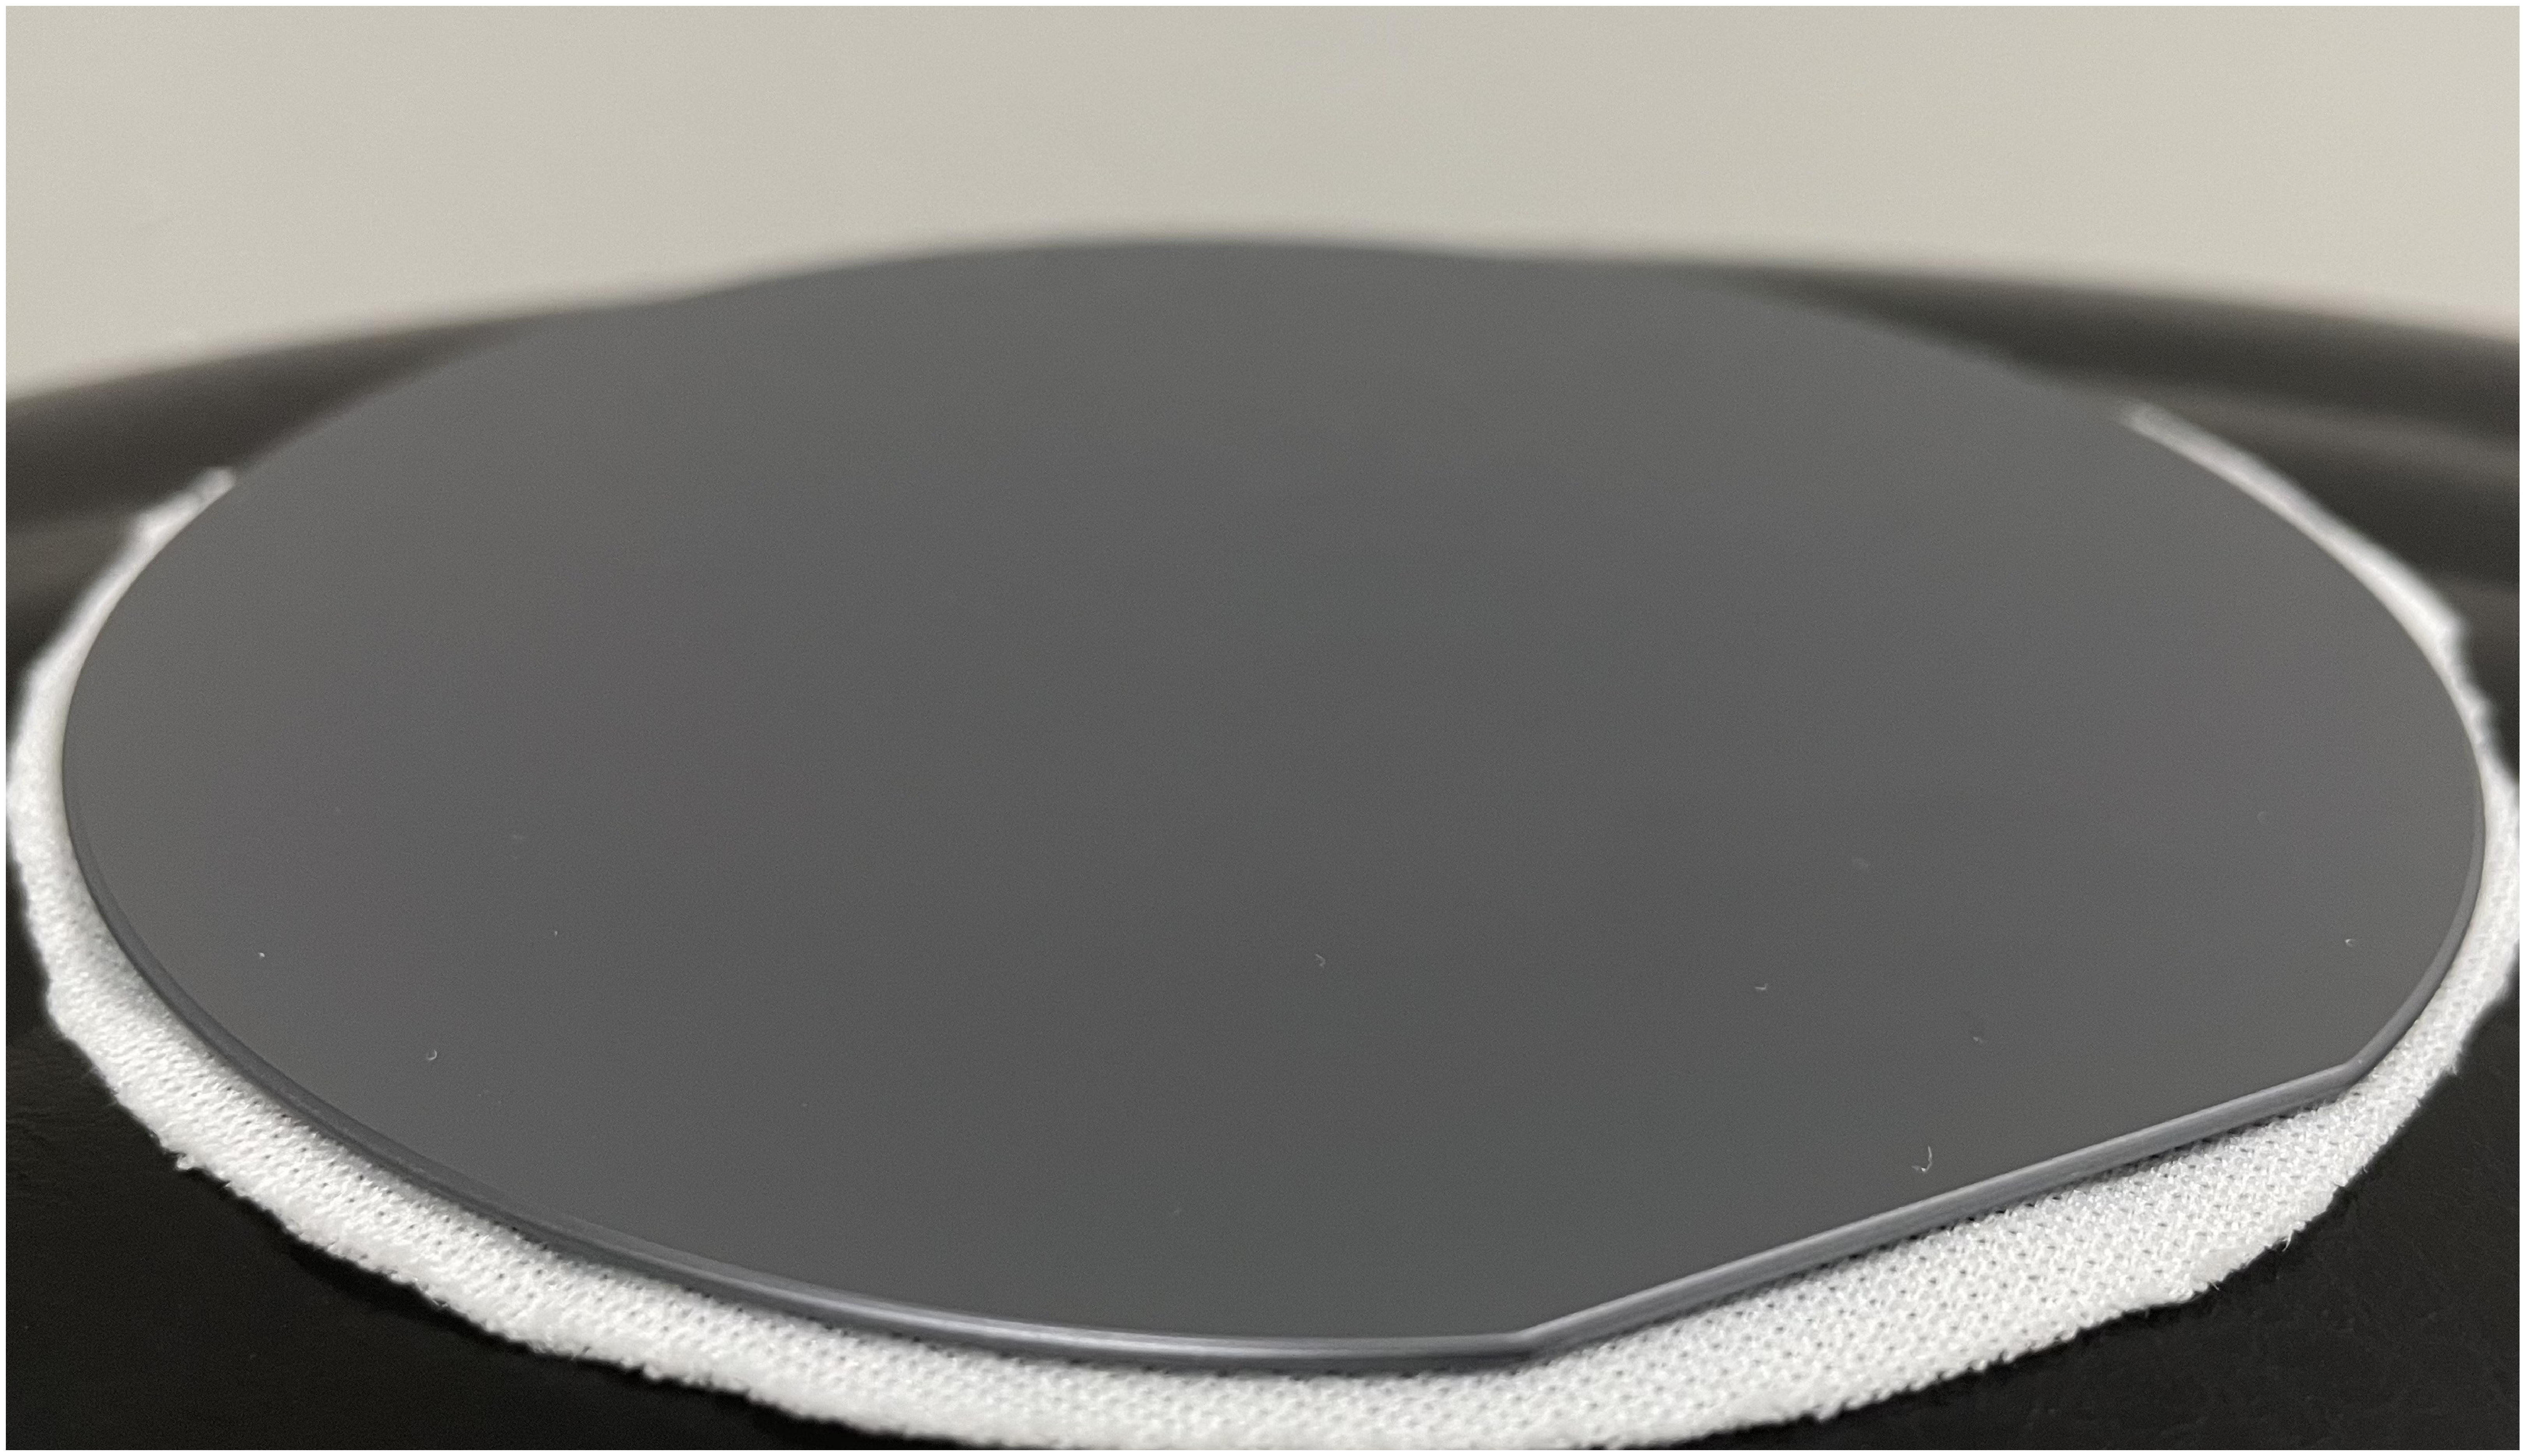
\includegraphics[width=0.7\textwidth]{wafer}
\caption[The 3-inch GaN-on-Si wafer]{The 3-inch GaN-on-Si wafer}
\label{fig:wafer}
\end{figure}

In this research, the 3-inch GaN-on-Si wafers \index{Wafer} have been successfully epitaxially grown on Si(111) substrates \index{Substrate} using Aixtron CCS 3×2 MOCVD, as shown in \autoref{fig:wafer}. The total thickness is about 1 \unit{\mm}, including Si(111) substrate, AlN/AlGaN multi-layer buffer layer, unintentionally doped (UID) GaN buffer layer, intrinsic GaN \index{Two-dimensional electron gas (2DEG)} 2DEG channel \index{Channel} layer, AlN barrier layer, AlGaN barrier layer and GaN cap layer. The grown wafer exhibits good electrical performance with 300 \unit{\ohm}/square sheet resistance, \num{1.00e13} \unit{\per\square\cm} carrier density, 2000 \unit{\square\cm/(Vs)} mobility \index{Electron mobility} and \SI{600}{\volt} breakdown \index{Voltage!breakdown voltage} voltage.

\subsection{Wafer dicing}

\begin{figure}[H] 
\centering    
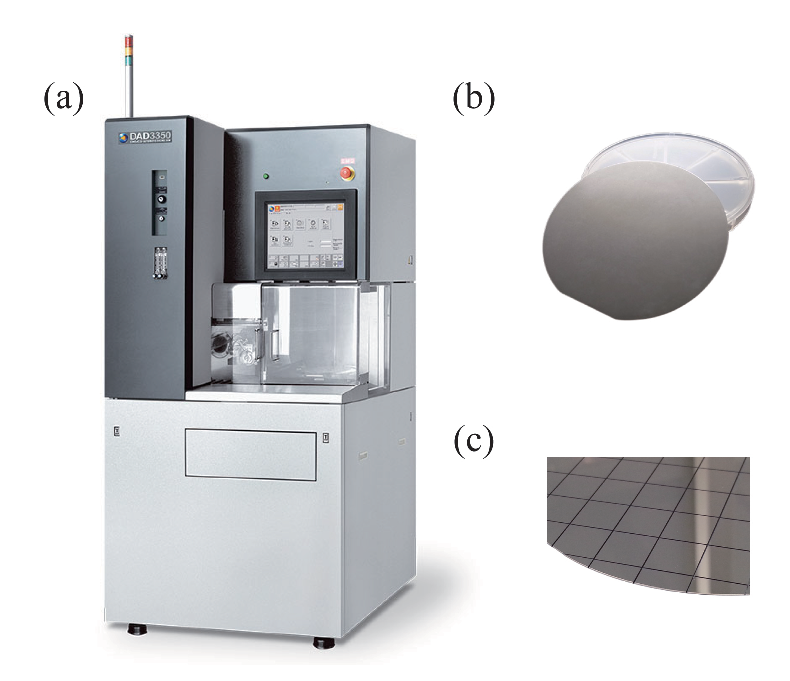
\includegraphics[width=0.8\textwidth]{CUT}
\caption[DISCO DAD3350 automatic dicing saw]{DISCO DAD3350 automatic dicing saw}
\label{fig:CUT}
\end{figure}

Compound semiconductors, such as GaN and SiC, are difficult to obtain high productivity with slow feed rates when using existing diamond blades for blade cutting, especially as wafer thickness becomes thinner. Therefore, utilizing beneficial characteristics of laser energy, laser cutting has developed as a highly promising method in dicing-grinding \index{Dice} service. Laser applications minimize kerf streets, thereby suiting special materials such as GaN or SiC when blade dicing reaches its limits. Further, working with laser technology provides a high degree of flexibility to die forms while offering high processing speed. Laser technology is developing rapidly and the semiconductor industry is taking full advantage of every innovation leap.

In this research, dice of size \numproduct{2 x 2} \unit{\mm} and \numproduct{3 x 3} \unit{\mm} have been cut from the grown 3-inch wafers \index{Wafer} with the DISCO DAD3350 automatic dicing saw.

\subsection{Cleaning technologies}
Cleaning procedures are essential steps in semiconductor processing. These are mostly used to remove particles and oxidize organic contaminants. Just a single particle on a \index{Wafer} wafer is enough to cause a killer defect or excursion that will ultimately lead to device failure. This is because both device reliability and final product yields are directly linked to the cleanliness of a wafer as it passes through the hundreds of patterning, etching, deposition and interconnect process steps. Therefore, the wafer must be strictly cleaned to remove organic and inorganic substances on the surface before the device fabrication process. The precondition of the cleaning process is not to destroy the surface characteristics of the epitaxial wafer. On this basis, the cleaning technologies, including wet cleaning and \index{Cleaning!dry cleaning} dry cleaning, are used to effectively remove various residual contaminants and impurities on the surface of the epitaxial \index{Surface} wafer. 

\begin{description}
	
\item [Wet cleaning] Some \index{Cleaning!wet cleaning} common cleaning solvents include acetone, trichloroethylene, ultrapure water, hydrochloric \index{Hydrochloric acid} acid, piranha solution, dilute HF \index{Hydrofluoric acid} solution and RCA cleaner. The cleaning steps of acetone, trichloroethylene, ultrapure water and hydrochloric acid are simple and will not be repeated. Piranha solution, dilute HF solution, and RCA cleaner are described as follows because of their better cleaning effect and certain dangers during the operation \cite{reinhardt2018handbook,king1998cleaning,tsujiwet}.

\begin{itemize}
\item[1.] Piranha solution

It consists of \ce{H2SO4} (98$\%$) and \ce{H2O2} (30$\%$) in different ratios, and is typically used for removing organic contaminants \index{Piranha solution} and \index{Photoresist} stripping photoresists.


\item[2.] RCA clean

The RCA clean \index{Wafer} is a \index{Cleaning!RCA cleaning} standard set of wafer cleaning steps which need to be performed before high-temperature processing steps (oxidation, diffusion, CVD) of wafers in semiconductor manufacturing. It involves the following chemical processes performed in sequence:

\begin{itemize}
	\item[2.1)] SC-1: organic clean + particle clean
	
	5 parts of deionized \index{Deionized water} water, 1 part of ammonia water, (29$\%$ by weight of \ce{NH3}), and 1 part of \index{Hydrogen peroxide} aqueous \ce{H2O2} (hydrogen peroxide, 30$\%$) at \SI{75}{\degreeCelsius} or \SI{80}{\degreeCelsius} typically for 10 minutes. This base-peroxide mixture removes organic residues. Particles are also very effectively removed, even insoluble particles. 
    
    \item[2.2)] SC-2: ionic clean
	
	6 parts of deionized water, 1 part of aqueous \index{Hydrochloric acid} HCl (hydrochloric acid, 37$\%$ by weight), and 1 part of aqueous \ce{H2O2} (hydrogen peroxide, 30$\%$)
at 75 or \SI{80}{\degreeCelsius} typically for 10 minutes. This treatment effectively removes the remaining traces of metallic (ionic) contaminants.
\end{itemize}

\item[3.] Dilute HF solution

Prepared by diluting 49$\%$ HF \index{Hydrofluoric acid} with dionized water (1:100) at room temperature and can effectively removes the oxide.

\end{itemize}

In this research, wet \index{Cleaning!wet cleaning} cleaning techniques have been applied to wafer \index{Wafer} cleaning, residual photoresist \index{Photoresist} removal, silicone oil cleaning, organic and particle contamination removal.


\begin{figure}[t] 
\centering    
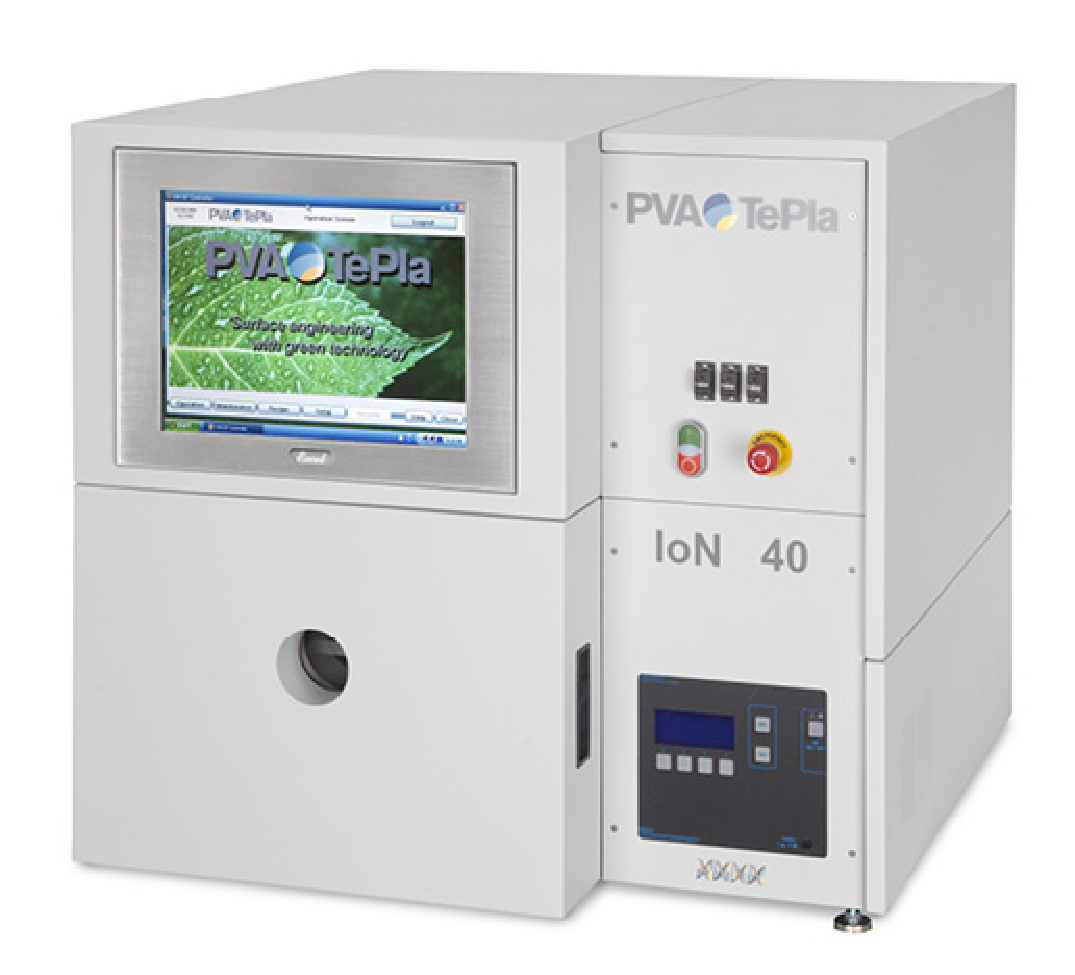
\includegraphics[width=0.6\textwidth]{plasma}
\caption[PVA TePla IoN 40 plasma cleaner]{PVA TePla IoN 40 plasma cleaner}
\label{fig:plasma}
\end{figure}

\item [Dry cleaning] Plasma technology is often characterized as a "dry" cleaning \index{Cleaning!dry cleaning} process, using ionized gases in vacuum chambers to remove all organic matter from the surface of the semiconductors through the use of an ionized gas called plasma. Plasma is an ionized gas capable of conducting electricity and absorbing energy from an electrical supply. Manmade plasma is generally created in a low-pressure environment. When a gas absorbs electrical energy, its temperature increases causing the ions to vibrate faster and "scrub" a \index{Surface} surface. This is generally performed in a vacuum chamber utilizing oxygen and/or argon gas and is an effective way to clean without using hazardous solvents. In contrast to chemically-based wet technologies, which have their role in removing thicker contaminants in the \index{Cleaning!plasma cleaning} micron range, plasma deals with contamination in the nanometer range on substrate and wafer surfaces.

In this research, PVA TePla IoN 40 plasma cleaner is mainly used to remove residual photoresist \index{Photoresist} and organic cleaning solutions by generating oxygen ions.
 
\end{description}

Cleaning technologies are crucial steps in the semiconductor manufacturing process and directly affects the performance and reliability of the device. In the process integration of \autoref{ch:Process Development and Integration of Power MEMS Devices}, a large number of cleaning processes can be found between lithography, etching, deposition, etc. They connect all processes as an indispensable intermediate link. The purpose of the cleaning process is to remove the residual influence of the previous process to the greatest extent on the premise of retaining the previous process results, and to provide a good operating environment for the subsequent process.

\subsection{Photolithography}

\begin{figure}[H] 
\centering    
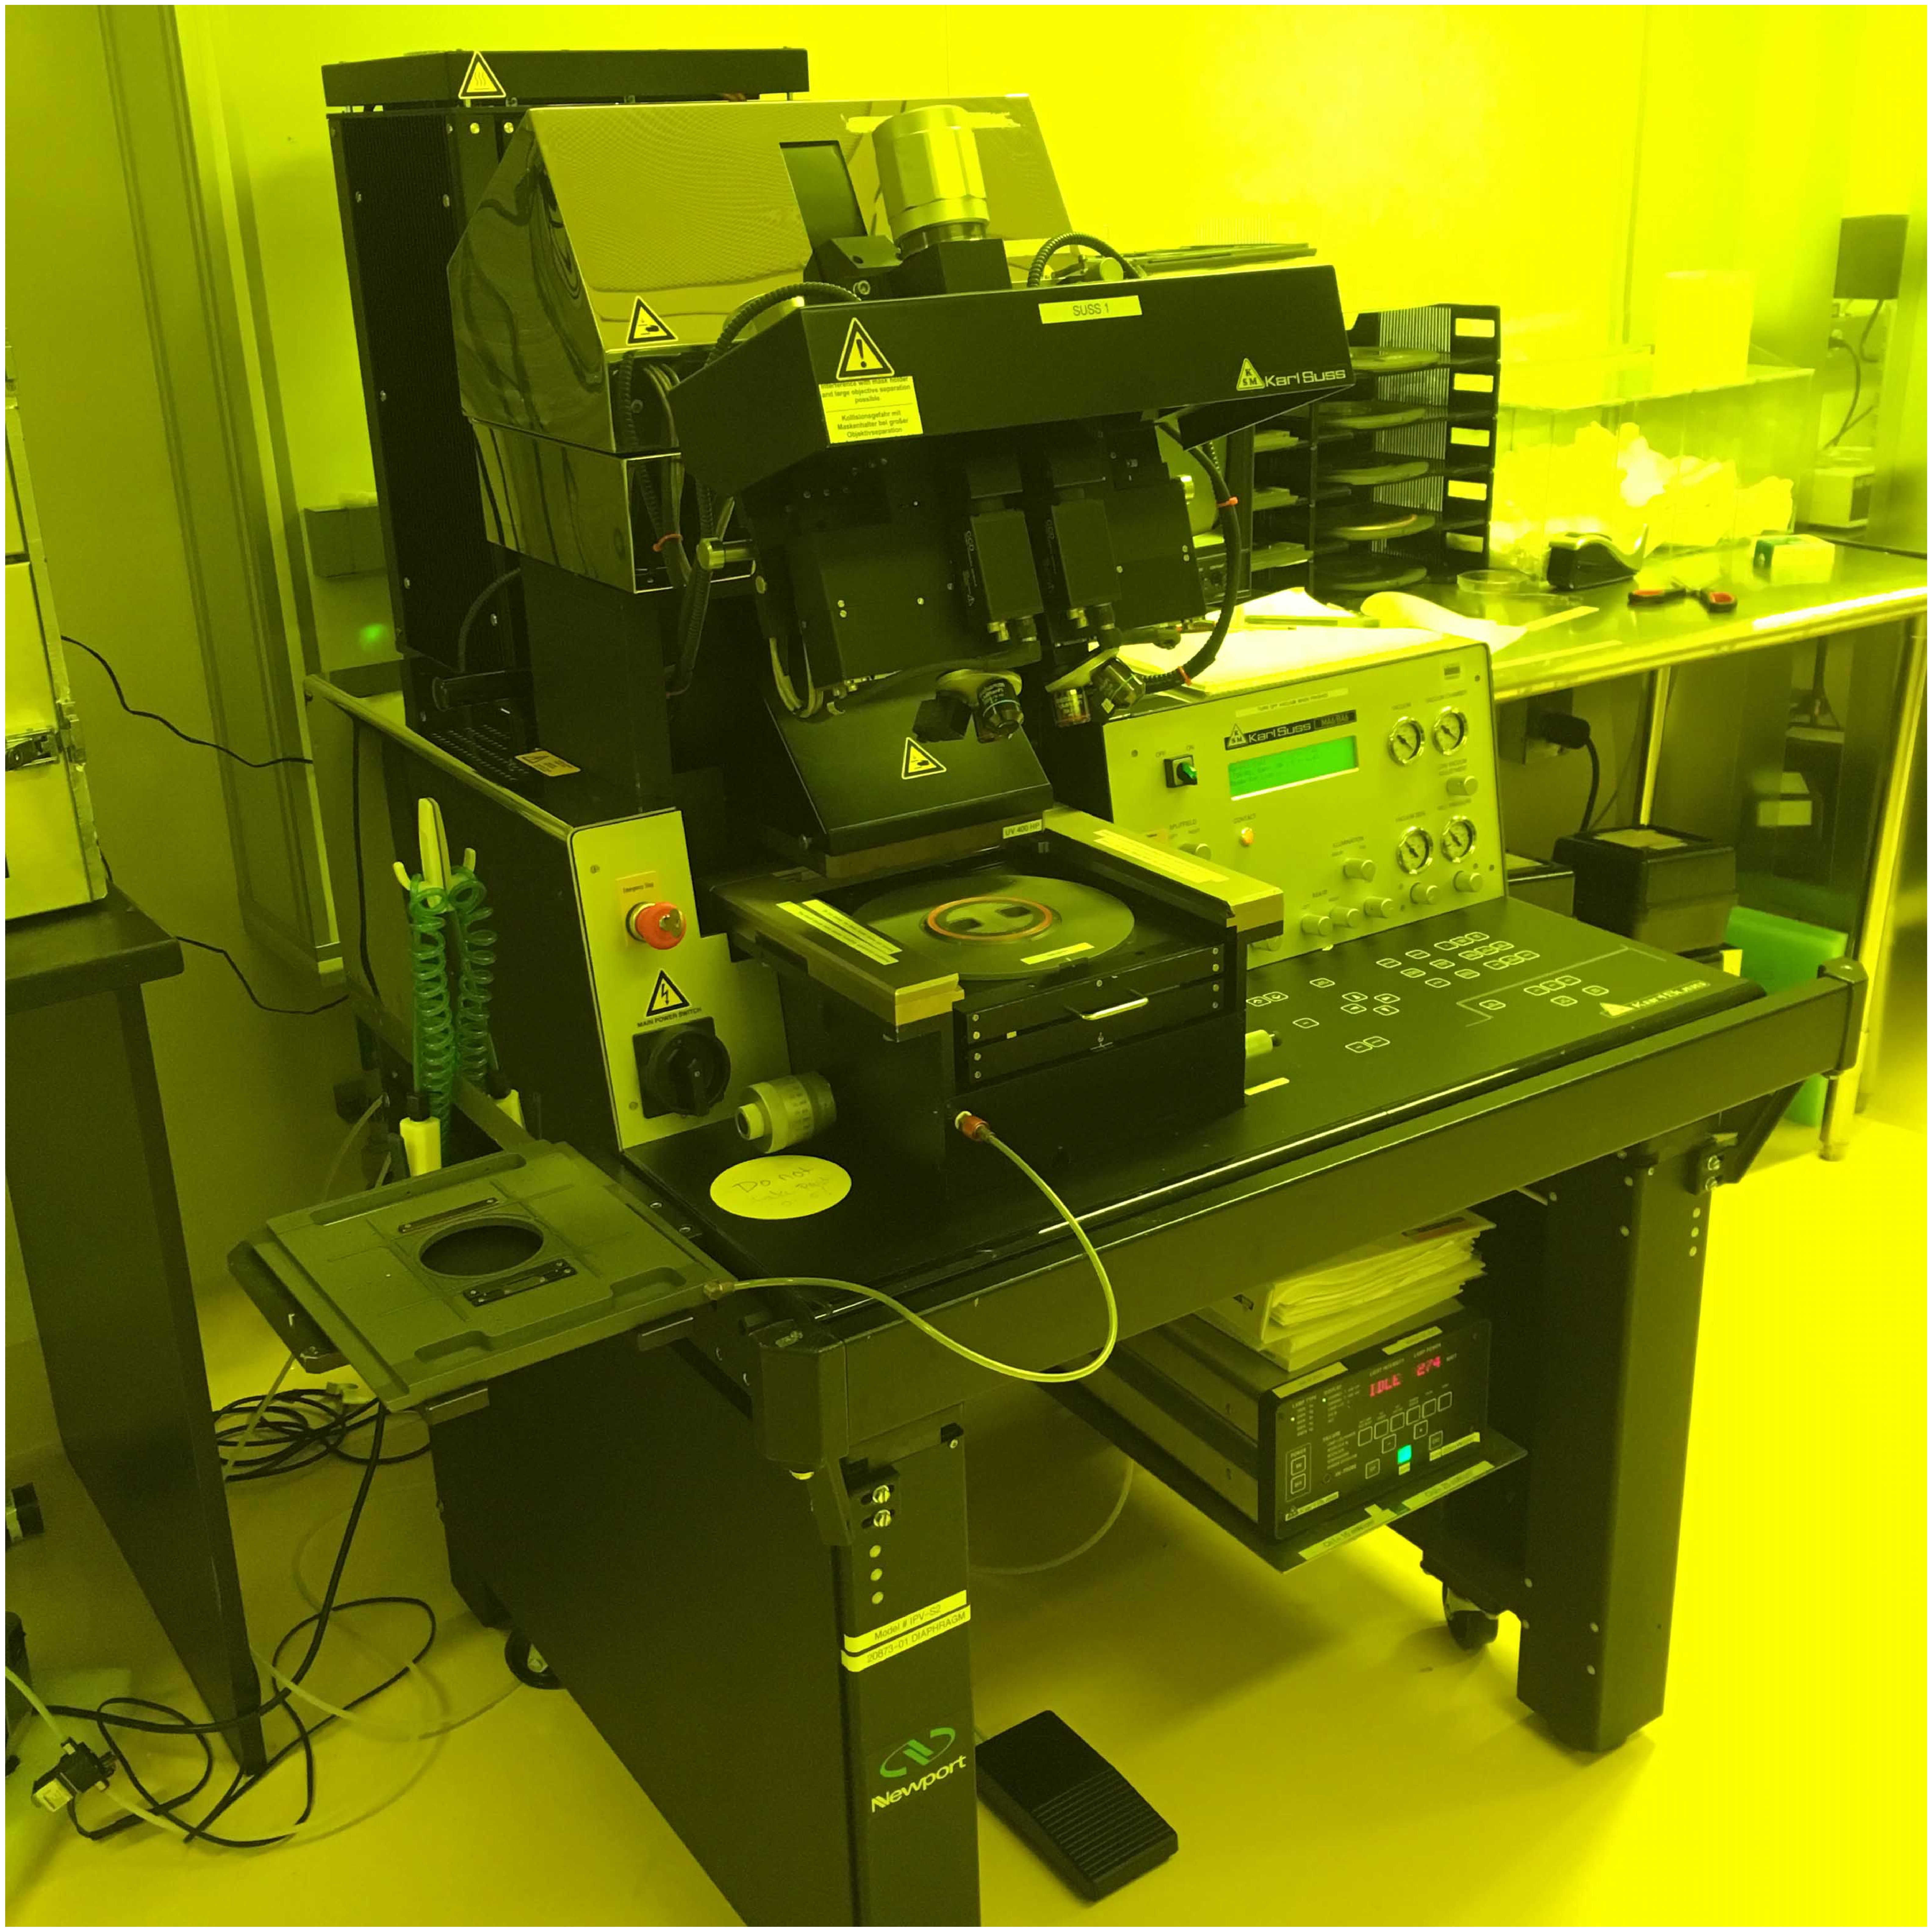
\includegraphics[width=0.6\textwidth]{photolithography}
\caption[SUSS MA6 mask aligner designed for high-resolution photolithography]{SUSS MA6 mask aligner designed for high-resolution photolithography}
\label{fig:photolithography}
\end{figure}

Photolithography \index{Photolithography} is an optical means of transferring a pattern on a \index{Substrate} substrate. It uses light to produce minutely patterned \index{Thin film} thin films of suitable materials over a substrate to protect selected areas of it during subsequent etching, deposition, or implantation operations. Typically, ultraviolet light is used to transfer a geometric design from an optical mask to a light-sensitive chemical \index{Photoresist} (photoresist) coated on the substrate. The photoresist either breaks down or hardens where it is exposed to light. The patterned film is then created by removing the softer parts of the coating with appropriate solvents.

The photolithography process is divided into positive photoresist and negative photoresist according to the type of photoresist. A negative photoresist is a type of photoresist in which the portion of the photoresist that is exposed to light becomes insoluble to the photoresist developer. The unexposed portion of the photoresist is dissolved by the photoresist developer. Whereas, a positive photoresist is a type of photoresist in which the portion of the photoresist that is exposed to light becomes soluble to the photoresist \index{Photoresist} developer. The unexposed portion of the photoresist remains insoluble to the photoresist developer.

\begin{figure}[H]
\centering    
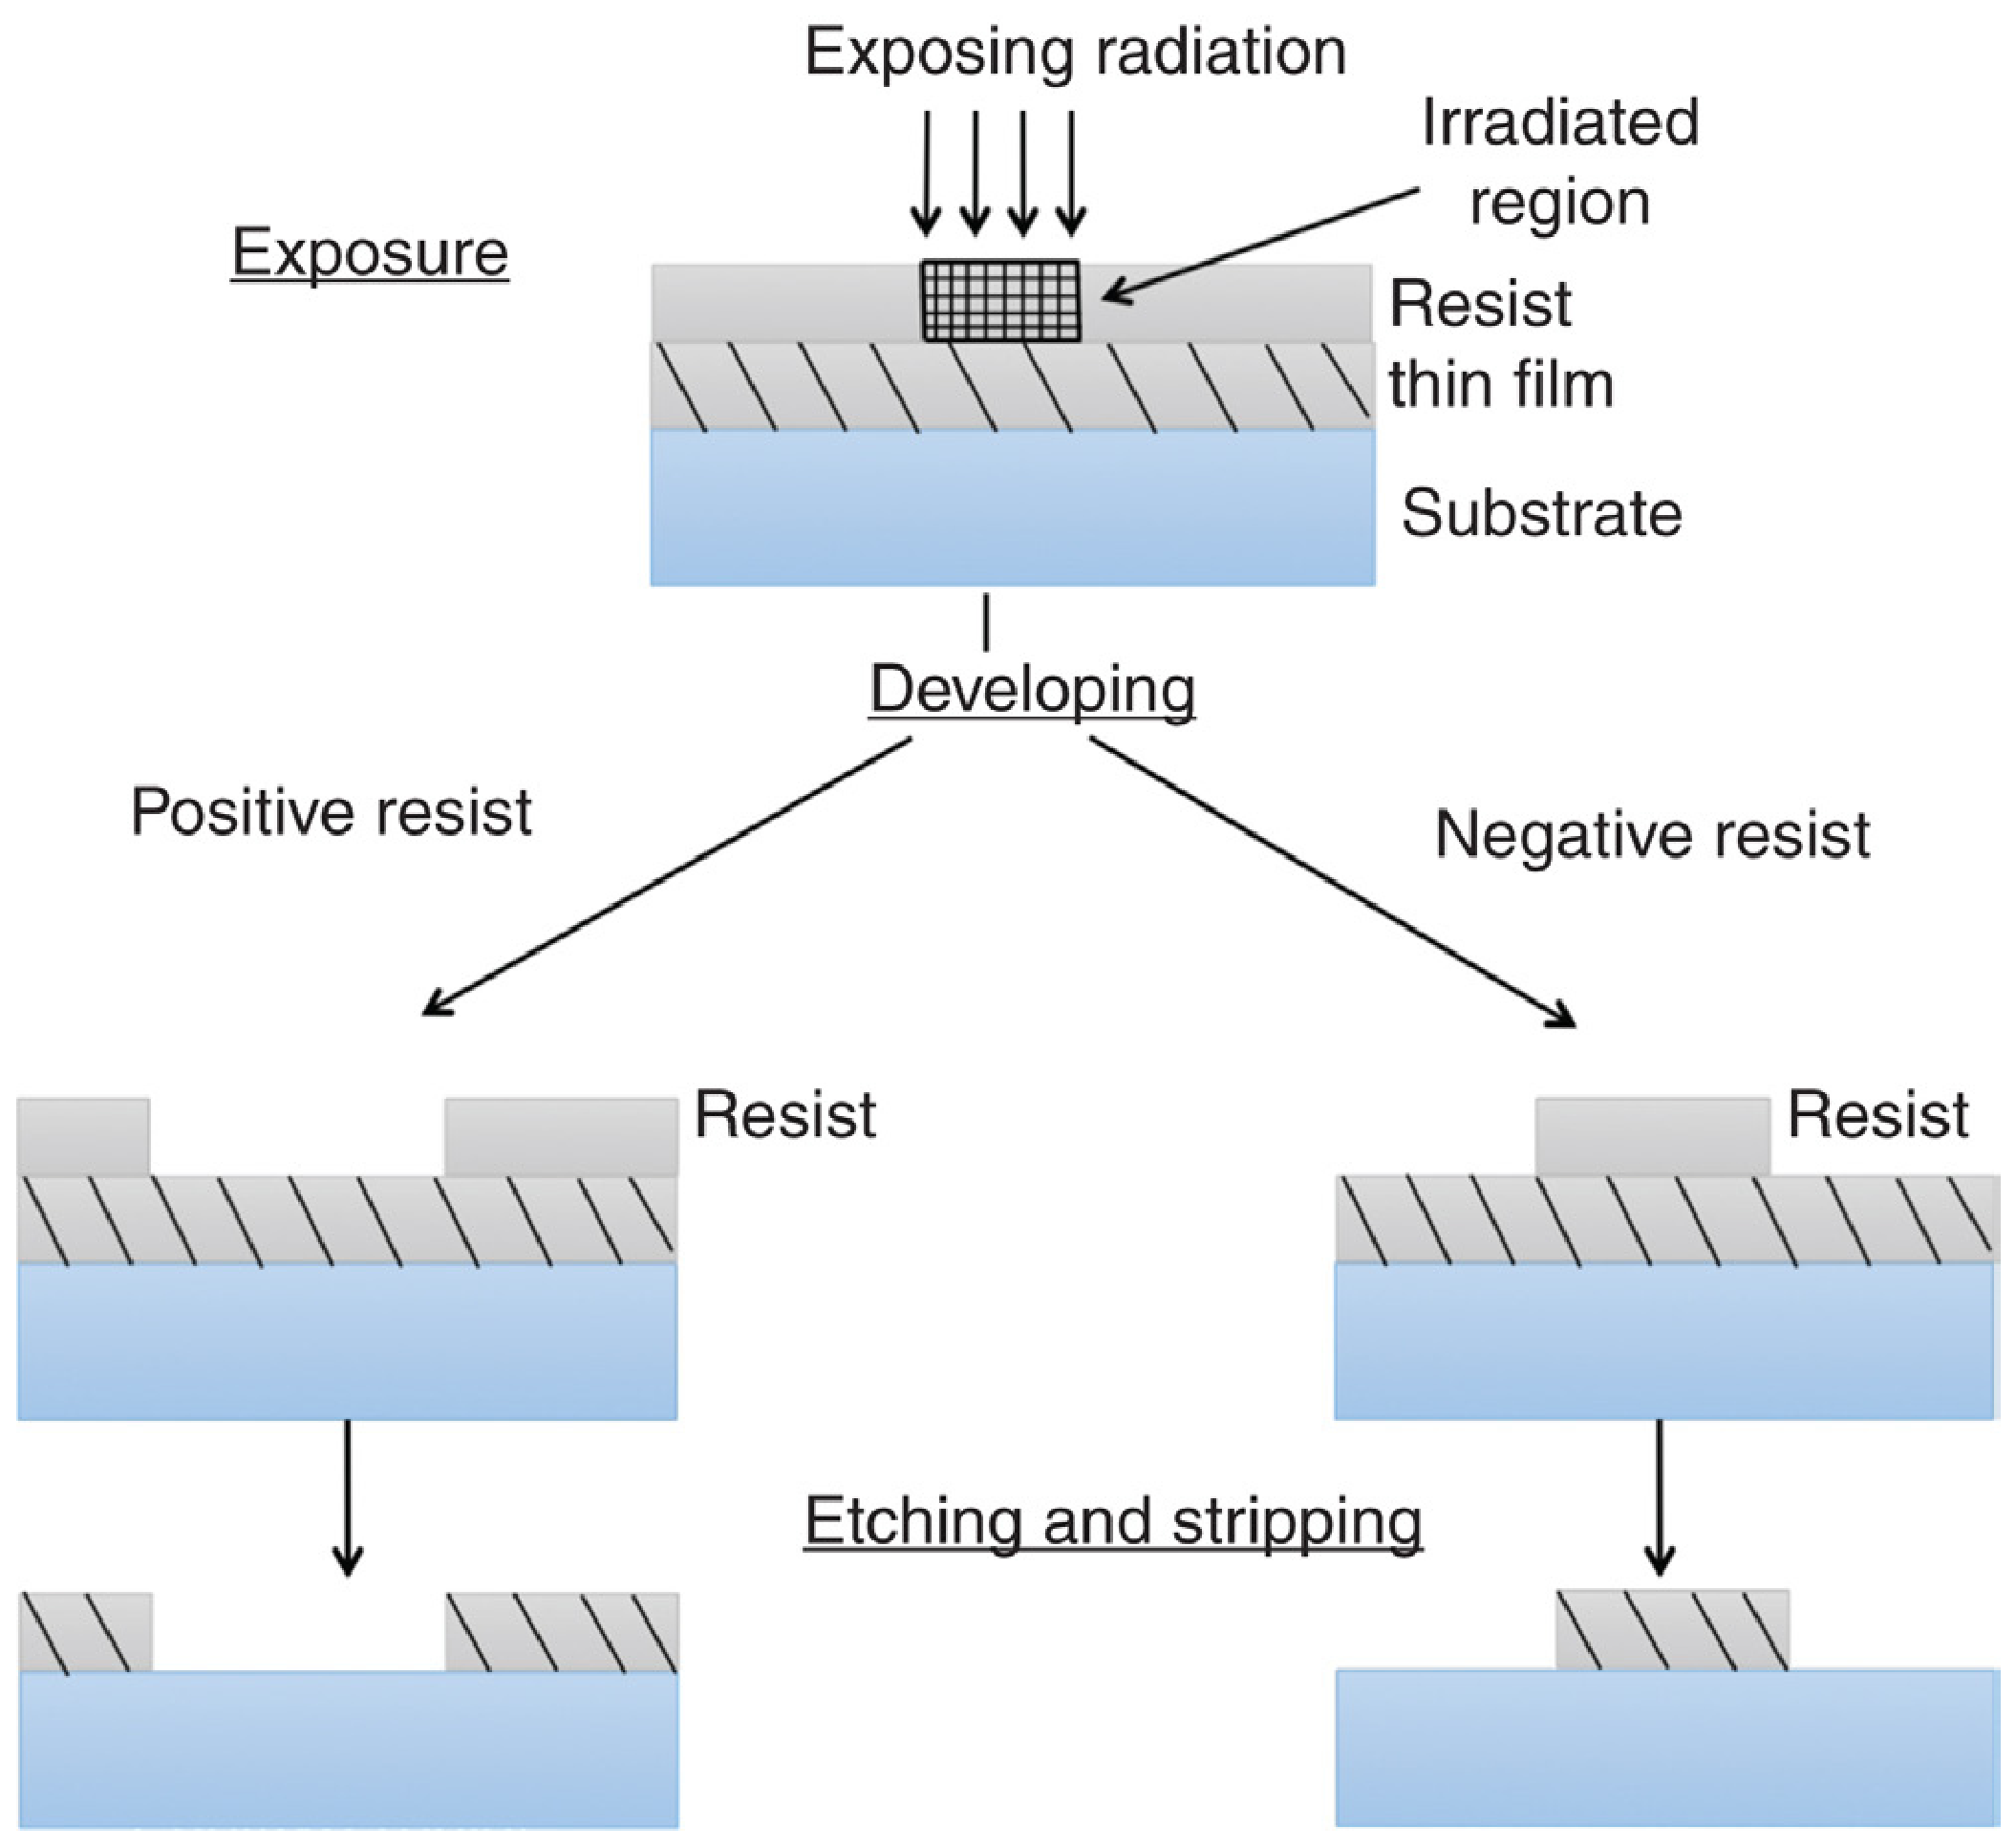
\includegraphics[width=0.6\textwidth]{photoprocess}
\caption[The schematic diagram showing the process of photolithography]{The schematic diagram showing the process of photolithography \cite{ram2018advanced}}
\label{fig:photolithography}
\end{figure}


In this research, the SUSS MA6 mask aligner designed for high-resolution photolithography at the micrometer scale has been applied to transfer patterns from mask to wafer, including mesa patterns, electrode \index{Electrode} patterns, cantilever \index{Cantilever} patterns, etc.

\subsection{Thin film deposition}

Thin Film deposition is the technology of applying a very thin film of material - between a few nanometers to about 100 micrometers, or the thickness of a few atoms – onto a "substrate" surface \index{Substrate} to be coated, or onto a previously deposited coating to form layers. Thin Film deposition is usually divided into two broad categories - chemical deposition and physical vapor deposition coating systems. Chemical deposition is that a volatile fluid precursor produces a chemical change on a surface leaving a chemically deposited coating, such as chemical vapor \index{Deposition!chemical vapor deposition (CVD)} deposition (CVD). Physical vapor deposition (PVD) \index{Deposition!physical vapor deposition (PVD)} refers to a wide range of technologies where a material is released from a source and deposited on a substrate \index{Substrate} using mechanical, electromechanical or thermodynamic processes. The two most common techniques of physical vapor deposition are thermal evaporation and sputtering.

\begin{figure}[H] 
\centering    
\includegraphics[width=0.9\textwidth]{magsup}
\caption[Denton Discovery 635 magnetron sputtering system]{Denton Discovery 635 magnetron sputtering system}
\label{fig:magsup}
\end{figure}

\begin{description}
	\item[Magnetron sputtering]
	
Sputter deposition \index{Deposition!magnetron sputtering} is a physical vapor deposition (PVD) method of thin film deposited by sputtering. The general sputtering method can be used to prepare a variety of materials such as metals, semiconductors, insulators, etc., and has the advantages of simple equipment, easy control, large coating area, and strong adhesion. Sputtering sources often employ magnetrons that utilize strong electric and magnetic fields to confine charged plasma particles close to the surface of the sputter target. In a magnetic field, electrons follow helical paths around magnetic field lines, undergoing more ionizing collisions with gaseous neutrals near the target surface than would otherwise occur. The sputter gas is typically an inert gas such as argon. The plasma can also be sustained at a lower pressure this way.  The certain target atoms near the surface gain sufficient momentum for outward motion and are sputtered out of the target and the sputtered atoms are neutrally charged and so are unaffected by the magnetic trap. These sputtered atoms deposit onto the surface \index{Surface} of the sample to form thin films.

Magnetron sputtering \index{Deposition!magnetron sputtering} includes direct current (DC) magnetron sputtering and radio frequency (RF) magnetron sputtering, each has a different working principle and application objects. The main advantage of RF magnetron sputtering over DC magnetron sputtering is that it does not require the target as an electrode be electrically conductive. Therefore, any material can be sputter-deposited theoretically using RF magnetron sputtering. Magnetron sputtering is advantageous as it doesn’t require evaporation or melting of source materials, allowing for exotic material experimentation and novel coating film applications. Sputter deposition is excellent for materials with high melting points that cannot be evaporated. It can achieve denser coatings than evaporation and is perfect for metallic or insulating coatings with specific optical or electrical properties.

\end{description}

\begin{figure}[H] 
\centering    
\includegraphics[width=0.9\textwidth]{ebeam}
\caption[Denton Vacuum Explore 14 electron beam evaporation system]{Denton Vacuum Explore 14 electron beam evaporation system}
\label{fig:ebeam}
\end{figure}

\begin{description}

	\item[Electron beam evaporation] 
		
E-beam (electron beam) evaporation \index{Deposition!electron beam evaporation} is a thermal evaporation process. E-beam evaporation provides for the direct transfer of a larger amount of energy into the source material, enabling the evaporation of metal and dielectric materials with very high melting temperatures, such as gold and silicon dioxide, respectively.  In e-beam evaporation, the evaporation material can be placed directly in a water-cooled copper hearth or into a crucible and heated by a focused electron beam. Electron beams can be generated by thermionic emission, field electron emission or the anodic arc method. The generated electron beam is accelerated to a high kinetic energy and directed towards the evaporation material. The thermal energy that is produced heats up the evaporation material causing it to melt or sublimate. Once temperature and vacuum level are sufficiently high, vapor will result from the melt or solid. The resulting vapor can then deposits on the substrate to form the required thin film

The deposition rate in this process can be as low as 1 nm per minute to as high as few micrometers per minute. The material utilization efficiency is high relative to other methods, and the process offers structural and morphological control of films, as well as the very high deposition rate. E-Beam evaporations are also advantageous for polymeric coating due to its simplicity and flexibility. E-Beam coatings also process in a more rapid fashion in a batch scenario as compared to Magnetron Sputtered coatings which make them ideal for high-volume commercial applications. E-Beam evaporations work for a wide variety of materials, including those with higher melting points that cannot undergo thermal evaporation, deliver better step coverage than sputtering or chemical vapor deposition (CVD), and offers a higher material utilization efficiency and higher deposition rates than sputtering.
	
\end{description}

In this research, the Denton Discovery 635 magnetron sputtering system has been applied to deposit the magnetic thin film \ce{(Fe90Co10)78Si12B10} in MPD, and the Denton Vacuum Explore 14 electron beam evaporation system has been used to deposit the ohmic and Schottky contact metals \index{Contact!Ohmic contact} in \index{Contact!Schottky contact} both SPD and MPD, including Ti, Al, Au and Ni.

\subsection{Dry etching}

\begin{figure}[H] 
\centering    
\includegraphics[width=0.9\textwidth]{icp}
\caption[SENTECH SI 500 inductively coupled plasma reactive ion etching]{SENTECH SI 500 inductively coupled plasma reactive ion etching}
\label{fig:icp}
\end{figure}


ICP RIE etching \index{Inductively coupled plasma (ICP)} is an advanced technique designed to deliver high etching rates, high selectivity and low damage processing. The gases are introduced above an inductive coil, placed around a ceramic tube. RF is applied to both the coil and chuck to create a plasma. The substrate is placed on the RF-powered chuck, and the wafer takes on potential which accelerates etching species extracted from plasma toward the etched surface. The introduction of different gases can produce different chemical reactions, thereby achieving the purpose of effectively etching different materials. Usually, \ce{SF6}/\ce{Ar}/\ce{O2} gas is used to etch Si and its compound materials, while \ce{BCl3}/\ce{Cl2}/\ce{Ar} gas is widely used to etch GaN and its compound materials. The etching rate can be effectively adjusted by the etching power. This technology combines chemical reaction and ion-induced etching to achieve a high degree of process flexibility. 

In this research, SENTECH SI 500 ICP-RIE plays an important role in the mesa isolation and cantilever \index{Cantilever} structure fabrication process. Especially in the preparation of the cantilever structure, by combining the process design of anisotropic etching \index{Etching!anisotropic etching} of GaN and isotropic etching \index{Etching!isotropic etching} of Si, the cantilevered \index{Cantilever} power MEMS devices with good uniformity and excellent performance has been successfully prepared. It can be determined that ICP-RIE process is the core process technology in the research of GaN power MEMS devices.

\subsection{Rapid thermal processing}

\begin{figure}[H] 
\centering    
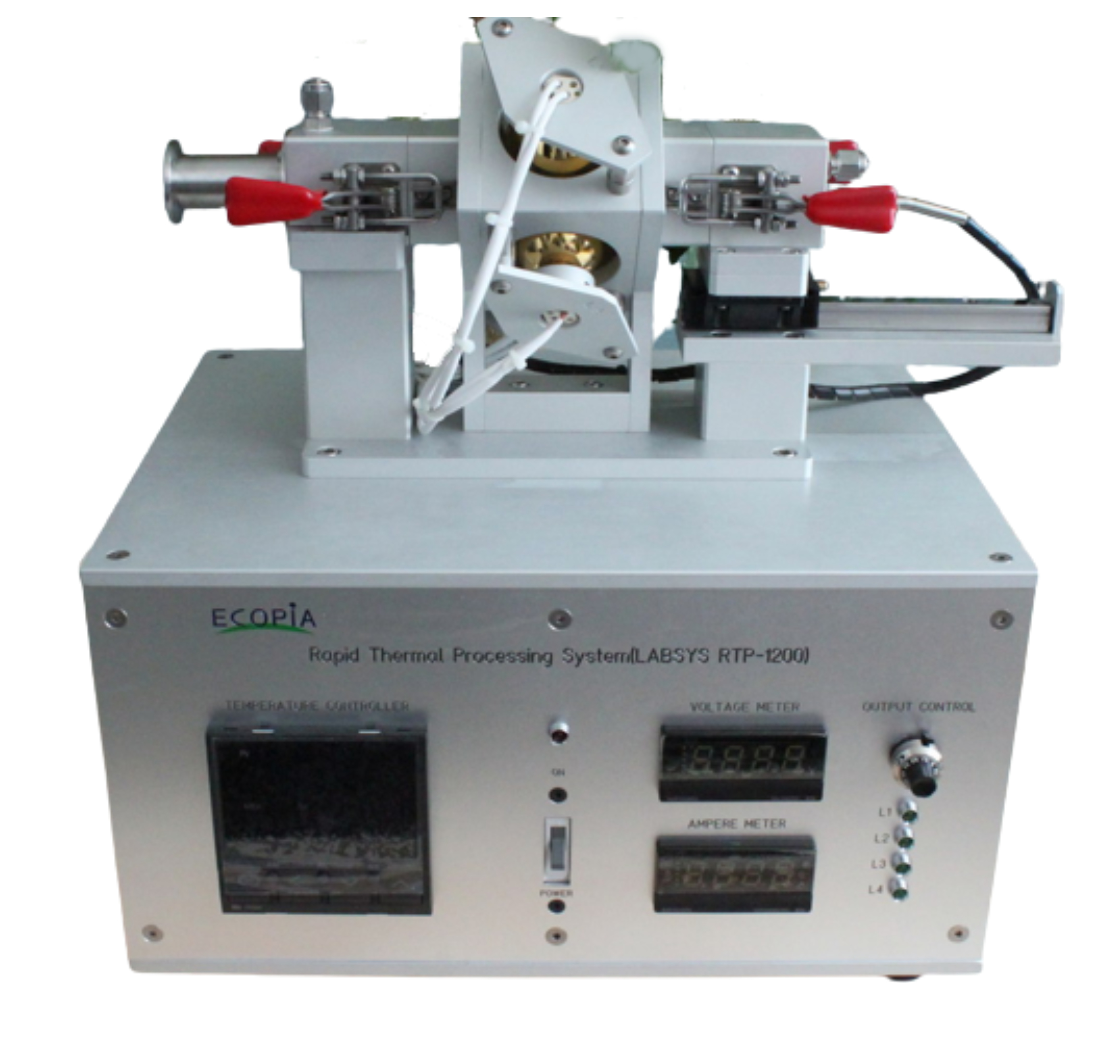
\includegraphics[width=0.5\textwidth]{RTP}
\caption[LABSYS RTP-1200 rapid thermal processing system]{LABSYS RTP-1200 rapid thermal processing system}
\label{fig:RTP}
\end{figure}

Rapid thermal processing (RTP) \index{Rapid thermal!processing (RTP)} is a semiconductor manufacturing process which heats silicon wafers to temperatures exceeding 1,000°C for not more than a few seconds. During cooling wafer temperatures must be brought down slowly to prevent dislocations and wafer breakage due to thermal shock. Such rapid heating rates are often attained by high-intensity lamps or lasers. These processes are used for a wide variety of applications in semiconductor manufacturing including dopant activation, thermal oxidation, metal reflow, silicide and barrier metal formation, chemical vapor deposition, and other steps in semiconductor manufacturing.

In this research, LABSYS RTP-1200 RTP is mainly used for ohmic contact formation in AlGaN/GaN HEMTs, and the most commonly used ohmic contact metal composition is Ti/Al/Ni/Au (from surface to bottom).


\section{Characterization techniques}

\subsection{Semiconductor parameter analyzer}

\begin{figure}[H] 
\centering    
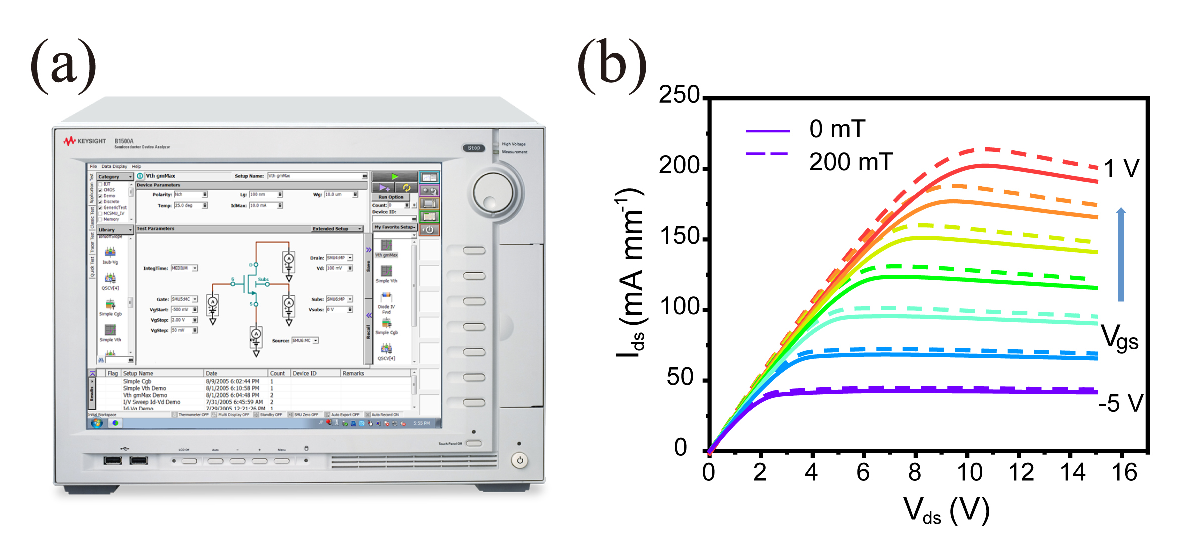
\includegraphics[width=0.9\textwidth]{keysight}
\caption[Keysight B1500A semiconductor device parameter analyzer and I-V characteristics of MPD under external magnetic field modulation]{Keysight B1500A semiconductor device parameter analyzer and I-V characteristics of MPD under external magnetic field modulation}
\label{fig:keysight}
\end{figure}

A semiconductor parameter analyzer \index{Semiconductor parameter analyzer} is an all-in-one unit designed to discover the characteristics of semiconductor devices such as diodes, transistors, and thyristors. Based on an oscilloscope, the device also contains voltage and current sources that can be used to stimulate the device under test. The function is to apply a swept (automatically continuously varying with time) voltage to the terminals of the device under test and measure the amount of current that the device permits to flow at each voltage. This V-I (voltage versus current) graph is displayed on an oscilloscope screen. Configuration includes the maximum voltage applied, the polarity of the voltage applied (including the automatic application of both positive and negative polarities), and the resistance inserted in series with the device. The main terminal voltage can often be swept up to several thousand volts, with load currents of tens of amps available at lower voltages.

For two terminal devices such as diodes, the parameter analyzer can display all of the interesting parameters such as the diode's forward voltage, reverse leakage current, reverse breakdown voltage, and so on. For three-terminal devices such as transistors and FETs also use a connection to the control terminal of the device being tested, and the control terminal current or voltage is stepped. By sweeping the voltage through the configured range of main terminal voltages, for each voltage step of the control signal, a group of I-V curves is generated automatically. The parameter analyzers can characterize the electrical characterization of the transistors, diodes, resistors and capacitors that make up semiconductors. 

In this research, the Keysight B1500A semiconductor device parameter analyzer has been widely used to test the electrical properties of AlGaN/GaN HEMTs and power MEMS devices, especially the I-V characteristics under external stimulus.
 

\subsection{Scanning electron microscopy (SEM)}

\begin{figure}[H] 
\centering    
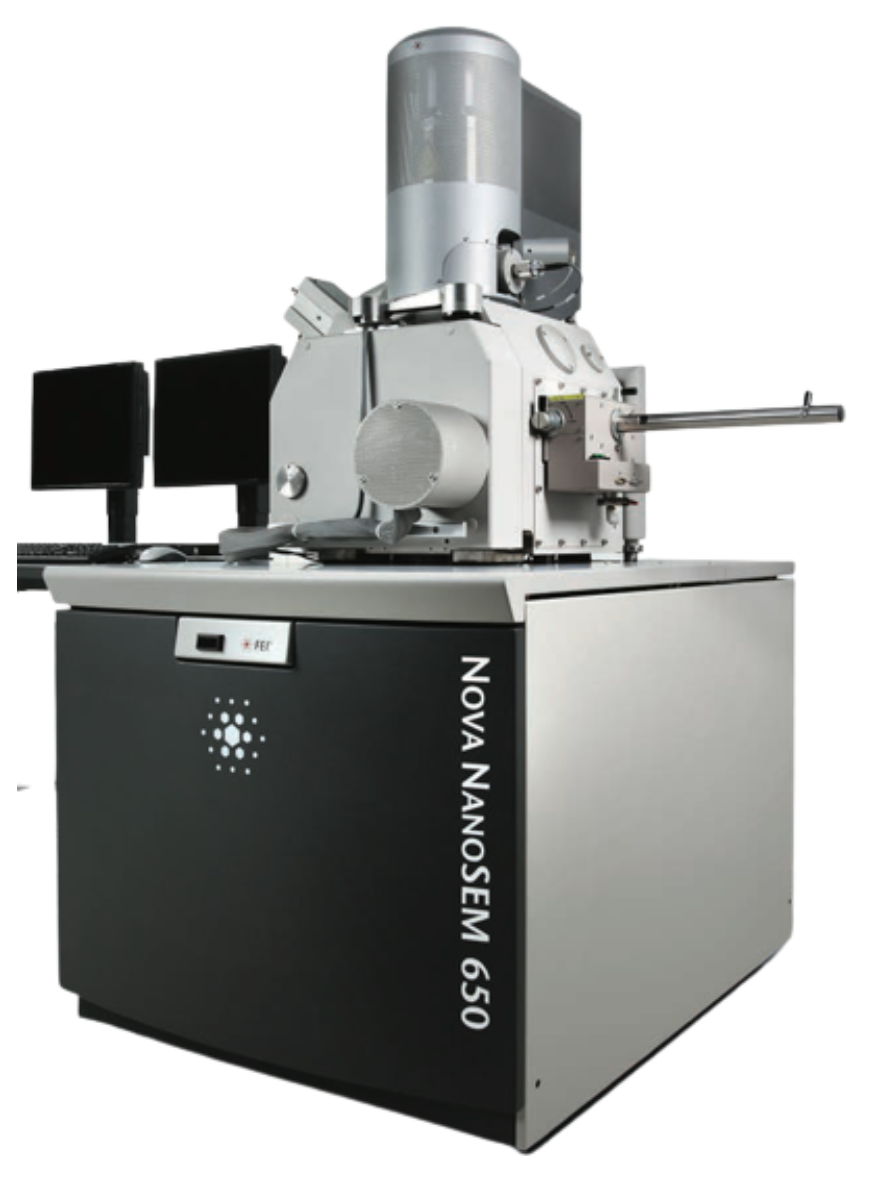
\includegraphics[width=0.45\textwidth]{sem}
\caption[FEI Nova Nano SEM 450 field-emission scanning electron microscopy]{FEI Nova Nano SEM 450 field-emission scanning electron microscopy}
\label{fig:sem}
\end{figure}

A scanning electron microscopy (SEM) \index{Scanning electron microscopy (SEM)} is a type of electron microscope that produces images of a sample by scanning the surface with a focused beam of electrons. The electrons interact with atoms in the sample, producing various signals that contain information about the surface topography and composition of the sample. The signals used by a SEM to produce an image result from interactions of the electron beam with atoms at various depths within the sample. Various types of signals are produced including secondary \index{Secondary electrons (SE)} electrons (SE), reflected or back-scattered electrons \index{Back-scattered electrons (BSE)} (BSE), and transmitted \index{Transmitted electrons} electrons. The electron beam is scanned in a raster scan pattern, and the position of the beam is combined with the intensity of the detected signal to produce an image. Due to the very narrow electron beam, SEM micrographs have a large depth of field yielding a characteristic three-dimensional appearance useful for understanding the surface structure of a sample. There is a wide range of magnifications, from about 10 times to more than 500,000 times, about 250 times the magnification limit of the best light microscopes. Some SEMs can achieve resolutions better than 1 nanometer \cite{reimer2000scanning}.

\begin{figure}[H] 
\centering    
\includegraphics[width=0.6\textwidth]{semgan}
\caption[SEM image of fabricated GaN power MEMS devices]{SEM image of fabricated GaN power MEMS devices}
\label{fig:semgan}
\end{figure}

In this research, FEI Nova Nano SEM 450 field-emission SEM can effectively obtain the topographic features of MEMS devices during fabrication, especially when dry-etching cantilever \index{Cantilever} structures. The accurate grasp of the topographic features greatly improves the efficiency of process development.

\subsection{Transmission electron microscopy (TEM)}

\begin{figure}[ht] 
\centering    
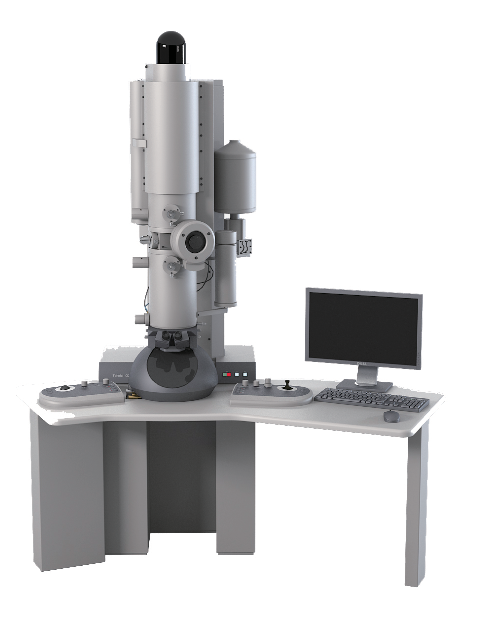
\includegraphics[width=0.5\textwidth]{TEM}
\caption[FEI Tecnai F20 cryo-transmision electron microscope]{FEI Tecnai F20 cryo-transmision electron microscope}
\label{fig:tem}
\end{figure}

Transmission electron microscopy (TEM) \index{Transmission electron microscopy (TEM)} is a microscopy technique in which a beam of electrons is transmitted through a specimen to form an image.  An image is formed from the interaction of the electrons with the sample as the beam is transmitted through the specimen. The image is then magnified and focused onto an imaging device. Transmission electron microscopes are capable of imaging at a significantly higher resolution than light microscopes, owing to the smaller de Broglie wavelength of electrons. This enables the instrument to capture fine detail—even as small as a single column of atoms, which is thousands of times smaller than a resolvable object seen in a light microscope.  What this means is that a TEM is capable of returning an extraordinary variety of nanometer- and atomic-resolution information, in ideal cases revealing not only where all the atoms are but what kinds of atoms they are and how they are bonded to each other. Transmission electron microscopy is a major analytical method in the physical, chemical and biological sciences and is widely used in materials science, nanotechnology and semiconductor research. 

The main difference between SEM and TEM is that SEM creates an image by detecting reflected or knocked-off electrons, while TEM uses transmitted electrons (electrons that are passing through the sample) to create an image. The magnifications that TEMs offer are much higher compared to SEMs. TEM can magnify the samples by more than 50 million times, while for the SEM, this is limited to 1-2 million times. As a result, TEM offers valuable information on the inner structure of the sample, such as crystal structure, morphology and stress state information, while SEM provides information on the sample’s surface and its composition.

\begin{figure}[ht] 
\centering    
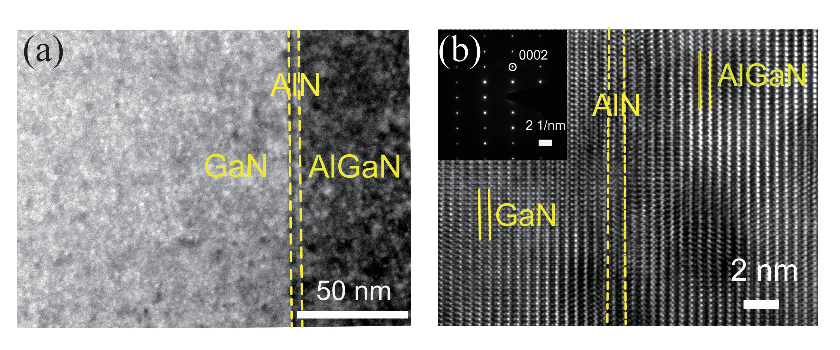
\includegraphics[width=0.9\textwidth]{TEMGaN}
\caption[High-resolution TEM image acquired from the AlGaN/AlN/GaN hetero-stacks]{High-resolution TEM image acquired from the AlGaN/AlN/GaN hetero-stacks}
\label{fig:temGaN}
\end{figure}

In this research, FEI Tecnai F20 TEM has been used to characterize the lattice orientation, lattice constants \index{Lattice!constant} and the dislocation defects of GaN, AlN, AlGaN layer.

\subsection{Energy dispersive X-ray spectroscopy (EDX)}

\begin{figure}[H] 
\centering    
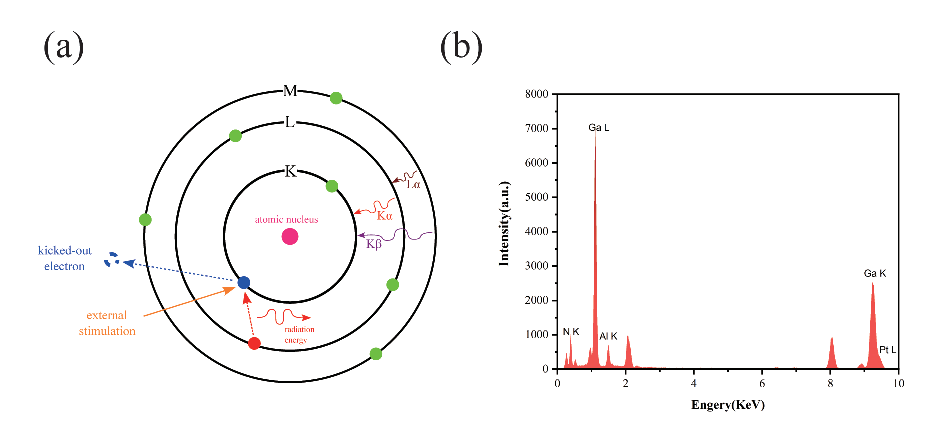
\includegraphics[width=0.9\textwidth]{edx}
\caption[Principle of EDX and elemental composition of AlGaN/GaN HEMT characterized by EDX]{Principle of EDX and elemental composition of AlGaN/GaN HEMT characterized by EDX}
\label{fig:edx}
\end{figure}

Energy-dispersive X-ray spectroscopy (EDS, EDX, EDXS or XEDS), \index{Energy-dispersive X-ray spectroscopy (EDX)} is an analytical technique used for the elemental analysis or chemical characterization of a sample. It relies on the interaction of some source of X-ray excitation and a sample. Its characterization capabilities are due in large part to the fundamental principle that each element has a unique atomic structure allowing a unique set of peaks on its electromagnetic emission spectrum. A beam of electrons is focused into the sample to stimulate the emission of characteristic X-rays from a specimen. At rest, an atom within the sample contains ground state (or unexcited) electrons in discrete energy levels or electron shells bound to the nucleus. The incident beam may excite an electron in an inner shell, ejecting it from the shell while creating an electron-hole where the electron was. An electron from an outer, higher-energy shell then fills the hole, and the difference in energy between the higher-energy shell and the lower-energy shell may be released in the form of an X-ray. The number and energy of the X-rays emitted from a specimen can be measured by an energy-dispersive spectrometer. As the energies of the X-rays are characteristic of the difference in energy between the two shells and of the atomic structure of the emitting element, EDS allows the elemental composition of the specimen to be measured \cite{goldstein2017scanning}.

In this research, the EDX equipment is integrated into the transmission electron microscopy equipment to characterize the elemental composition and distribution of AlGaN/GaN HEMTs.

\subsection{High-resolution X-ray diffraction (HRXRD)}

\begin{figure}[ht] 
\centering    
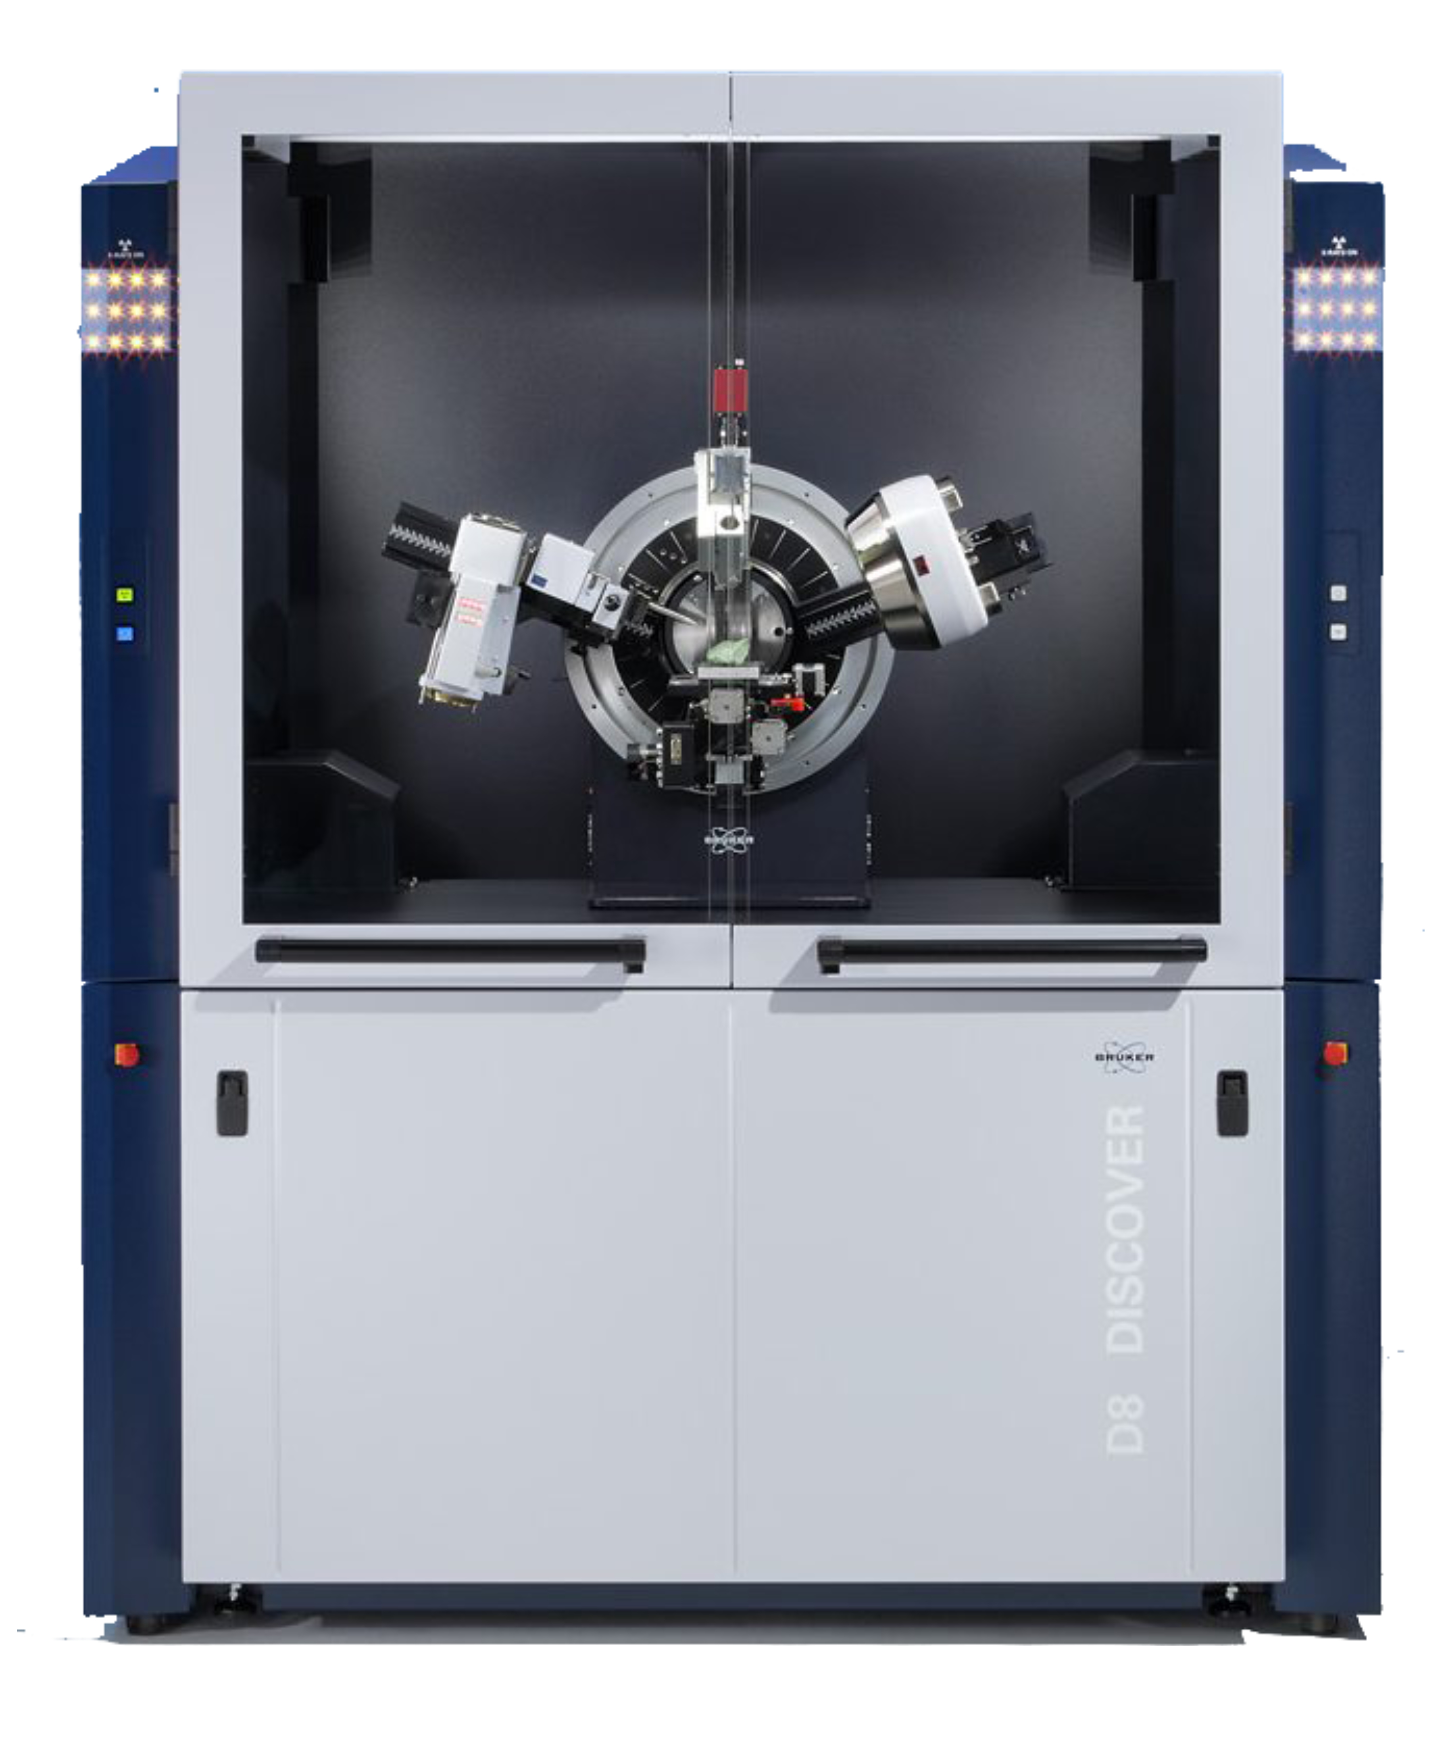
\includegraphics[width=0.6\textwidth]{xrd}
\caption[Bruker D8 DISCOVER high-resolution X-ray diffraction]{Bruker D8 DISCOVER high-resolution X-ray diffraction}
\label{fig:xrd}
\end{figure}

Most of today’s modern semiconductor device structures are epitaxially grown from the gas phase onto a substrate made from silicon, silicon-germanium, III-V and II-VI compounds. These films are nearly-perfect crystalline films containing a relatively low dislocation density. Film properties are largely determined by their compositional and structural parameters. Information such as layer thickness, composition, strain, relaxation and structural quality is obtained by measuring rocking curves and reciprocal space maps using high-resolution X-ray \index{High-resolution X-ray diffraction (HRXRD)} diffraction (HR-XRD). The spatial distribution of defects can also be visualized by X-ray diffraction imaging methods.

The working principle behind HRXRD is \index{Bragg’s law} Bragg’s law, which states that when the x-ray incident onto a crystal surface with an angle of incidence it will reflect back with a same angle of scattering When the path difference is equal to a whole number of wavelength, a constructive interference will occur. The path difference is the separation between the crystal \index{Crystal} planes that caused the reflection. The crystalline structure causes a beam of incident X-rays to diffract into many specific directions. By measuring the angles and intensities of these diffracted beams, HRXRD can be used to analyze the thickness, composition, and strain state of epitaxial single-crystal thin films, and can also measure the density of defects in epitaxial layers by FWHM of Bragg reflections obtained in the direction perpendicular to the diffraction vector.

\begin{figure}[ht] 
\centering    
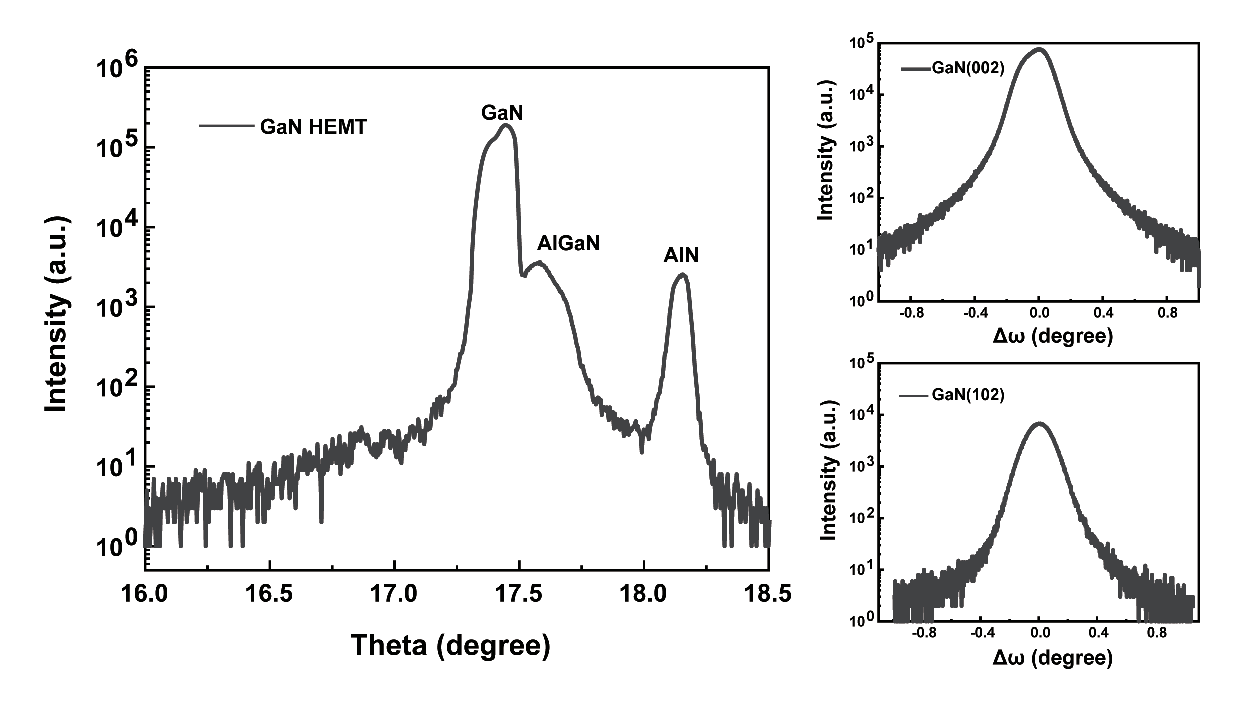
\includegraphics[width=0.9\textwidth]{xrdhemt}
\caption[The X-ray diffraction spectra of GaN HEMT]{The X-ray diffraction spectra of GaN HEMT}
\label{fig:xrdhemt}
\end{figure}

In this research, Bruker D8 DISCOVER HR-XRD has been used to measure the composition, defects and thickness of GaN Wafer.

\subsection{Raman spectroscopy}

\begin{figure}[H] 
\centering    

\includegraphics[width=0.9\textwidth]{raman}
\caption[HORIBA LabRAM HR Evolution Raman spectroscopy]{HORIBA LabRAM HR Evolution Raman spectroscopy}
\label{fig:raman}
\end{figure}

Raman scattering \index{Raman!scattering} is an extremely powerful contactless tool which allows non-destructive and quantitative microanalysis of structural and electrical properties of semiconductor materials. This technique is very useful since the Raman signal is very sensitive to the microstructural state of the sample and other local environments, therefore giving information on the structure of the material on the scale of a few lattice \index{Lattice!constant} constants. 

 Raman is a light scattering technique, whereby a molecule scatters incident light from a high-intensity laser light source. Most of the scattered light is at the same wavelength as the laser source and does \index{Rayleigh scattering} not provide useful information – this is called Rayleigh Scattering. However, a small amount of light (typically 0.0000001$\%$) is scattered at different wavelengths, which depend on the chemical structure of the analyte – this is called Raman \index{Raman!scattering} Scattering. Raman signal is a function of the electron-phonon interaction, i.e. lattice vibration. A Raman spectrum features a number of peaks, showing the intensity and wavelength position of the Raman scattered light. Each peak corresponds to a specific lattice vibration. Raman spectroscopy \index{Raman!spectroscopy} probes the chemical structure of a material and provides information about chemical structure and identity, phase and polymorphism, intrinsic stress/strain and contamination and impurity \cite{smith2019modern}.
 
\begin{figure}[H] 
\centering    
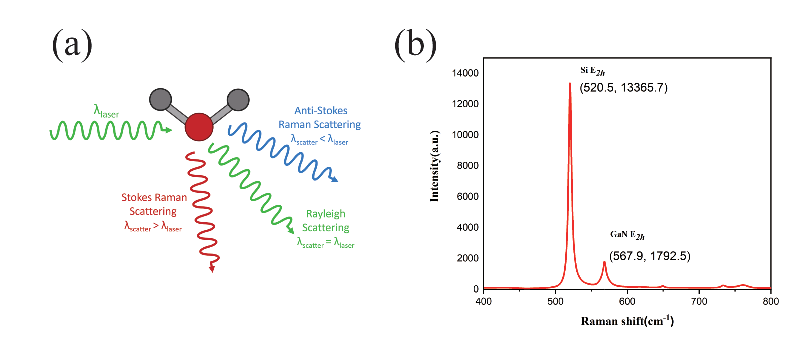
\includegraphics[width=1\textwidth]{ramanGaN}
\caption[Principle of Raman spectroscopy and Raman spectroscopy of GaN-on-Si wafers]{Principle of Raman spectroscopy and Raman spectroscopy of GaN-on-Si wafers}
\label{fig:ramangan}
\end{figure}

In this research, changes in the intrinsic lattice strain between AlGaN, AlN, and GaN layers during the fabrication of MEMS devices can be detected by HORIBA LabRAM HR Evolution Raman spectroscopy, which would greatly affects the material properties and electrical properties of MEMS devices.


\section{Summary}

In this chapter, a brief overview of the semiconductor fabrication and characterization equipment used in the manufacturing of GaN power MEMS is given. The equipment is briefly classified according to different functions such as deposition, etching, lithography, etc., and the specific models of the equipment, the basic working principle and the main use in this research are described. The independent processes of these devices with different functions are integrated to complete the preparation of GaN power MEMS, which becomes the basis of process integration in \autoref{ch:Process Development and Integration of Power MEMS Devices}.


\nomenclature[z-TEM]{TEM}{Transmission electron microscopy}
\nomenclature[z-SEM]{SEM}{Scanning electron microscopy}
\nomenclature[z-HAADF-STEM]{HAADF-STEM}{High-angle annular dark-field scanning transmission electron microscopy}
\nomenclature[z-EDX]{EDX}{Energy dispersive X-ray spectroscopy}
\nomenclature[z-MOCVD]{MOCVD}{Metal organic compound chemical vapor deposition}
\nomenclature[z-MOVPE]{MOVPE}{Metal organic vapor phase expitaxy}
\nomenclature[z-ICP-RIE]{ICP-RIE}{Inductively coupled plasma reactive ion etching}
\nomenclature[z-CVD]{CVD}{chemical vapor deposition}
\nomenclature[z-PVD]{PVD}{Physical vapor deposition}
\nomenclature[z-XRD]{XRD}{X-ray diffraction}
\nomenclature[z-RTP]{RTP}{Rapid thermal processing}
\nomenclature[z-UV]{UV}{Ultraviolet}
\nomenclature[z-EUV]{EUV}{Extreme ultraviolet}
\nomenclature[z-E-Beam]{E-Beam}{Electron beam}
\nomenclature[z-DC]{DC}{Direct current}
\nomenclature[z-RF]{RF}{Radio frequency}
\nomenclature[z-UID]{UID}{Unintentionally doped}

